\documentclass[10pt,a4paper]{article}
\usepackage[UTF8]{ctex}
\usepackage{fontspec}
\usepackage{geometry} 
\usepackage{amsmath}
\usepackage[shortlabels]{enumitem}
\usepackage{float}
\usepackage{graphicx}
\usepackage{subfigure}
\usepackage{epstopdf}
\usepackage{amsmath,amssymb}
\usepackage{diagbox}
\DeclareSymbolFont{EulerExtension}{U}{euex}{m}{n}
\DeclareMathSymbol{\euintop}{\mathop} {EulerExtension}{"52}
\DeclareMathSymbol{\euointop}{\mathop} {EulerExtension}{"48}
\let\intop\euintop
\let\ointop\euointop

\geometry{left=3.17cm,right=3.17cm,top=2.53cm,bottom=2.54cm}
%\setmainfont{Times New Roman}
\pagestyle{plain}
\setlist[enumerate,1]{label=\textbf{\arabic*.}}
\setlist[enumerate,2]{label=(\arabic*)}

\begin{document}

\begin{enumerate}

    \begin{figure}[H]
        \centering
        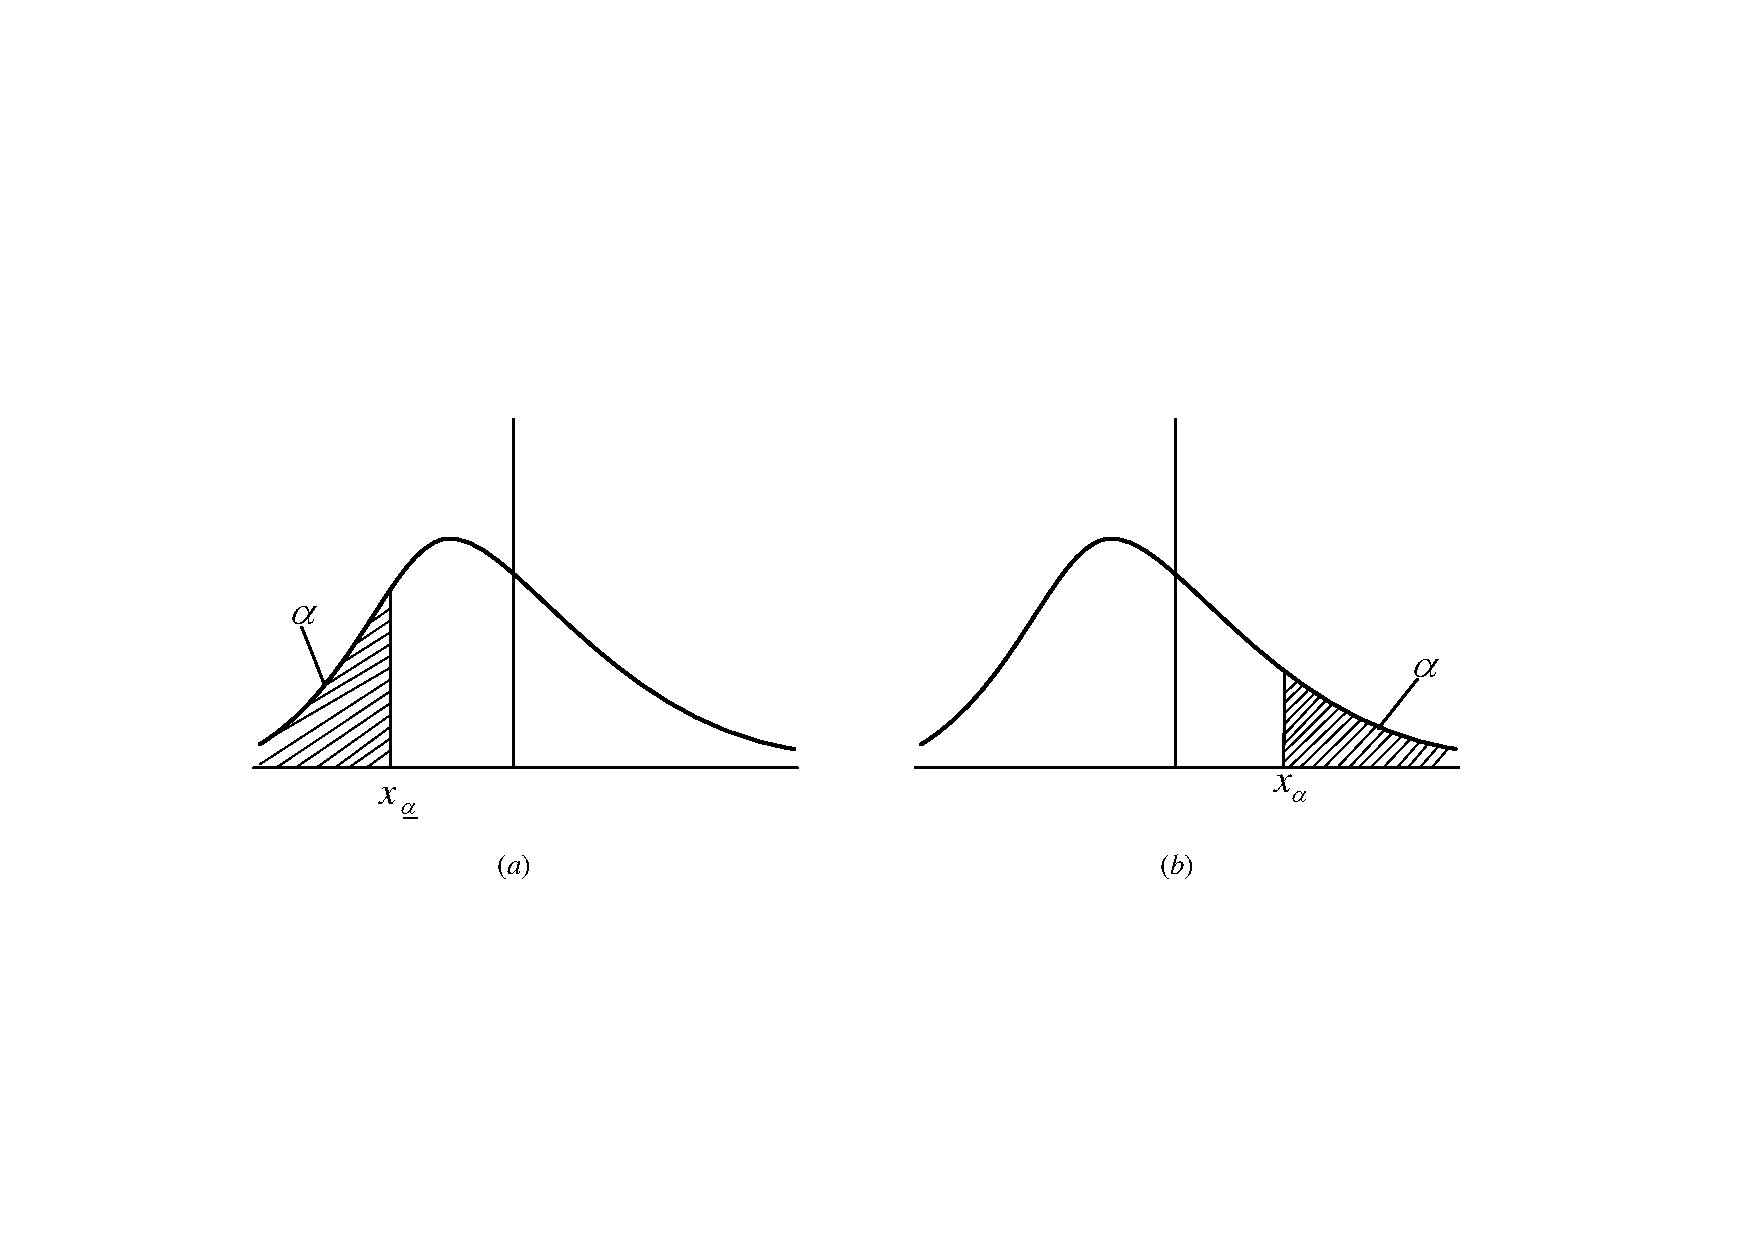
\includegraphics[width=0.8\textwidth]{4.38.pdf}
        \end{figure}
    
    % \begin{table}[H]\centering
    %     \begin{tabular}{c|cccccc}
    %     \hline
    %     \diagbox{$Y$}{$X$}  & 0    & 1    & 2    & 3    & 4    & 5    \\ \hline
    %     0 & 0.00 & 0.01 & 0.03 & 0.05 & 0.07 & 0.09 \\
    %     1 & 0.01 & 0.02 & 0.04 & 0.05 & 0.06 & 0.08 \\
    %     2 & 0.01 & 0.03 & 0.05 & 0.05 & 0.05 & 0.06 \\
    %     3 & 0.01 & 0.02 & 0.04 & 0.06 & 0.06 & 0.05 \\ \hline
    %     \end{tabular}
    % \end{table}

    \item 

  

\end{enumerate}
\end{document}